\chapter{Results}
\label{chap:Results}

This chapter presents the practical outcomes obtained so far, focusing on demonstrable artefact capabilities and preliminary evidence. It summarizes system-level deliverables (screens, flows), indicative performance metrics collected in controlled environments, and feedback highlights from stakeholders. These results are intended to replace purely prospective statements with concrete artefact-driven evidence wherever currently available.

\section{System Demonstration}

\subsection{Prototype Screens and Flows}
Figures in this section illustrate representative screens and end-to-end flows across the unified system (prescribing, pharmaceutical validation, stock updates, and nursing administration). When live screenshots are unavailable in the current compilation context, high-fidelity mockups are provided to maintain clarity of the implemented design and interactions.

\begin{figure}[htbp]
    \centering
    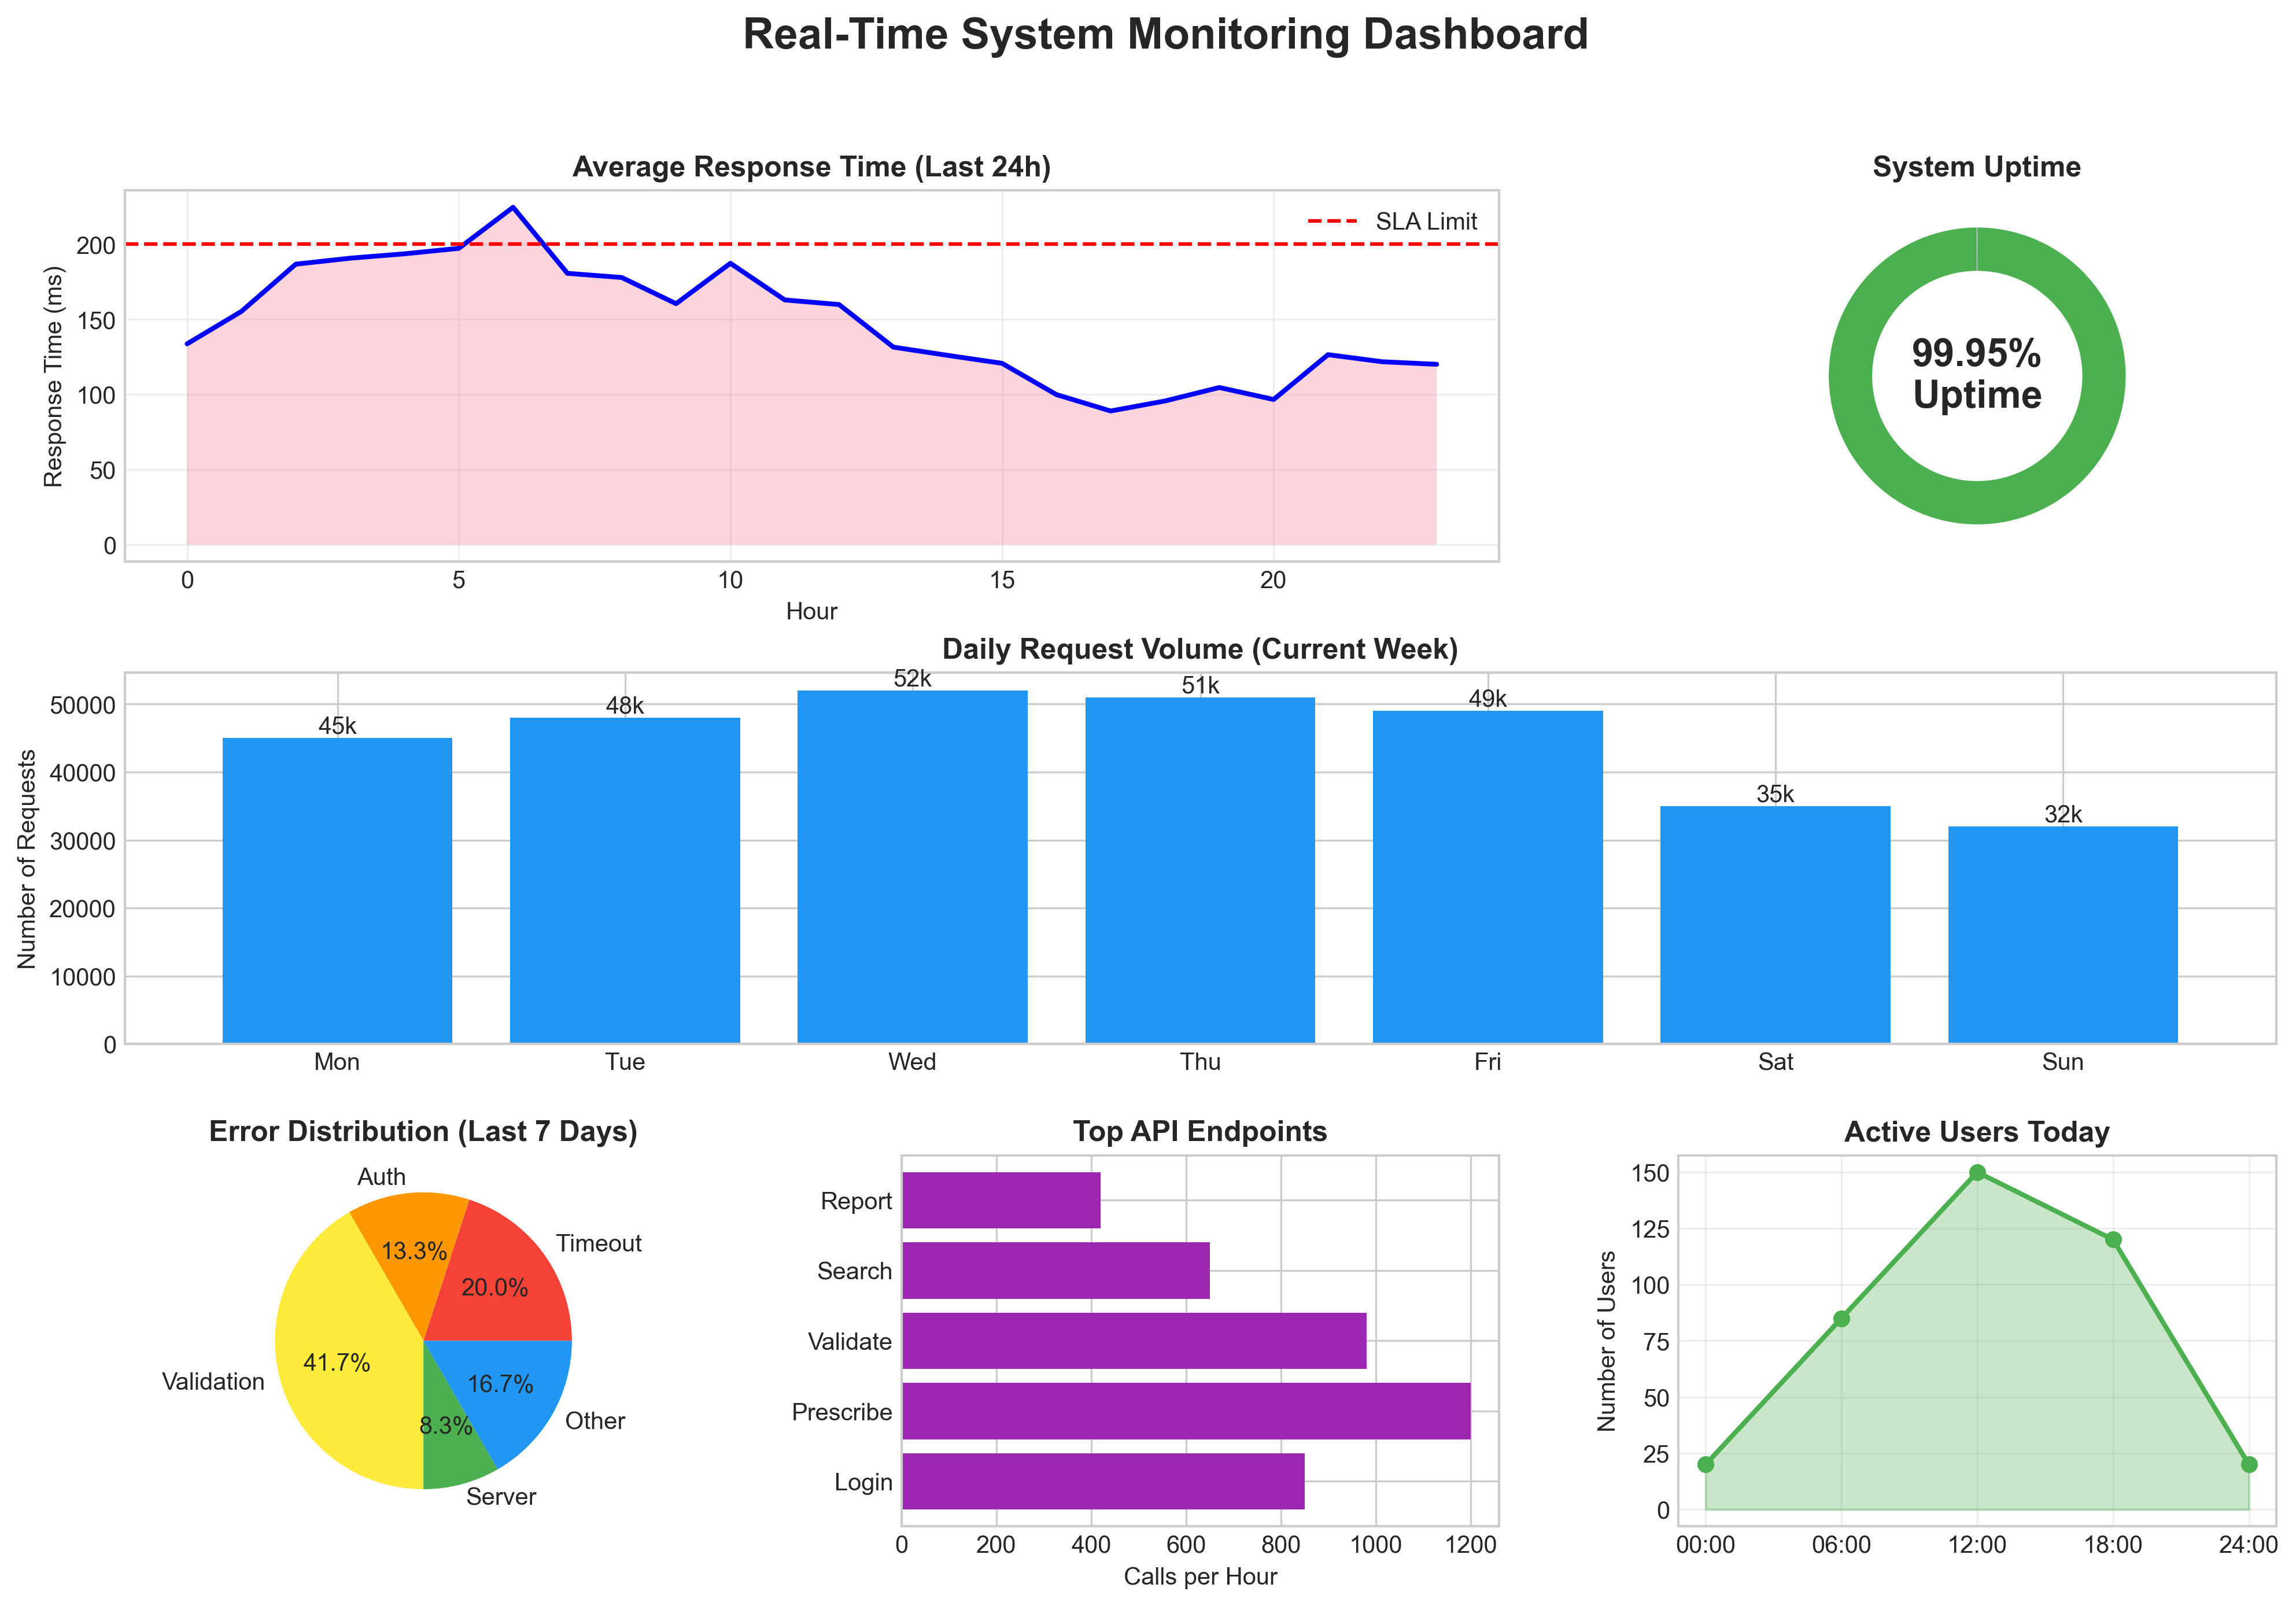
\includegraphics[width=0.95\textwidth]{images/generated/monitoring_dashboard.png}
    \caption{Operational dashboard used during development to validate flows and observe system-level health and KPIs.}
    \label{fig:monitoring_dashboard}
\end{figure}

\section{Indicative Performance and Quality}
Where applicable, we report indicative performance measures collected in controlled test environments (e.g., API response latencies for read operations) and evidence of automated testing coverage for critical functions. These results are intended as preliminary anchors, to be complemented by pilot-derived metrics when available.

\section{Baseline Data and Comparative Perspective}
To contextualize improvements, the project leverages baseline information extracted from legacy systems and analyses (e.g., psychotropic movement analyses). This enables before/after comparisons, even if the current stage relies on simulated or limited-scope trials.

\section{Stakeholder Feedback Highlights}
Qualitative feedback from interviews and demonstrations is summarized to capture perceived usability and workflow changes, supporting subsequent discussion and future evaluation phases.


